\section{A Minimal Model of Nutrient-Mediated Growth Rate Control}
While the preceeding subsections highlight a dominant role for ribosomes in
setting the growth rate, our analysis on the whole emphasizes that the total
proteomic content must change in response to variable growth conditions and
growth rate. In this final section we use a minimal model of growth rate control
to better understand how this interconnection between ribosomal abundance and
total protein influences the observed growth rates across the proteomic data.

Here we propose that cells modulate their proteomic composition in direct
response to the availability of nutrients in the growth media. As noted earlier,
bacteria can modulate ribosomal activity through the secondary-messenger
molecules like (p)ppGpp in poorer nutrient conditions (\FIG{ribosome_limit}(C) -
inset; \cite{dai2016}). Importantly, these molecules also cause global changes in
transcriptional and translational activity \citep{hauryliuk2015, zhu2019,
Buke2020}. In \textit{E. coli}, amino acid starvation causes the accumulation of
de-acylated tRNAs at the ribosome's A-site and leads to a strong increase in
(p)ppGpp synthesis activity by the enzyme RelA \citep{hauryliuk2015}. There is
also increasing evidence that (p)ppGpp can inhibit the initiation of DNA
replication \citep{kraemer2019}, resulting in a lower $\langle$\# ori$\rangle$
per cell in poorer growth conditions \citep{fernandezcoll2020}.


%
%  These observations raise the possibility that
% it is through (p)ppGpp that cells mediate the growth-rate dependent changes in
% $\langle$\# ori$\rangle$, cell size, and ribosomal abundance and activity
% . Indeed, recent work in a (p)ppGpp deficient strain of
% \textit{E. coli} found that cells exhibited $\langle$\# ori$\rangle$ and cell
% sizes that were more consistent with a fast growth state where (p)ppGpp levels
% are normally low . In this final section, we consider
% the interconnection between proteomic composition and ribosome abundance by
% formulating a minimal model of growth rate control. We use it to quantitatively
% show how tuning these parameters help cells maximize growth rate for a
% particular environment.

% The drastic changes observed in cell size, proteomic composition, and
% ribosome abundance across different growth conditions suggests a hypothesis
% that each parameter is being tuned to better match the cell's biosynthetic
% capacity to the specific environment.


% \subsubsection{Ribosomal Elongation Rate and Cellular Growth Rate are Linked by
% Amino Acid Scarcity}
% Here we consider a mode of regulation in which the rate of peptide elongation
% $r_t$ depends only on the availability of amino acids (and, therefore, also
% amino-acyl tRNAs). It is through the elongation rate $r_t$ that we assume cells
% adjust their ribosomal content ($R$, $\Phi_R$) according to nutrient
% availability.
%  and for simplicity, do not explicitly model changes in  $\langle$\#
% ori$\rangle$ or regulation by (p)ppGpp.

To impose this quantitatively, we assume that cells modulate their proteome
($N_\text{pep}$, $R$, $\Phi_R$) to better maximize their rate of peptide
elongation $r_t$.  Here, $r_t$ will depend on how quickly the ribosomes can
match codons with their correct amino-acyl tRNA, along with the subsequent steps
of peptide bond formation and translocation. This ultimately depends on the
cellular concentration amino acids, which we treat as a single effective
species, $[AA]_\text{eff}$. In our model, we determine the the rate of peptide
elongation $r_t$ and achievable growth rate as simply depending on the supply of
amino acids (and, therefore, also amino-acyl tRNAs), through a parameter
$r_{AA}$ in units of AA per second, and the rate of amino acid consumption by
protein synthesis ($r_t \times R \times f_a$). This is shown schematically in
\FIG{elongation_rate_model}(A) and derived in Appendix XX. Given our observation
that protein synthesis on the whole and energy production are not limiting, we
assume that other molecular players required by ribosomes like elongation
factors and GTP are in sufficient abundance.

% We therefore coarse-grain the steps of
% elongation to two time-scales,  1) the time required to find and bind each
% correct amino-acyl tRNA, and 2) the remaining steps in peptide elongation that
% will not depend on the amino acid availability. The availability of amino acids
% will depend on their cellular concentration, which we treat as a single
% effective species, $[AA]_\text{eff}$. The time to translate each codon is given
% by the inverse of the elongation rate $r_t$, which can be written as,
%
% \begin{equation}
% \frac{1}{r_t} = \frac{1}{k_{on} \alpha [AA]_{\text{eff}}} + \frac{1}{r_{t}^{\text{max}}}.
% \end{equation}
% where we have assumed that the rate of binding by amino-acyl tRNA $k_{on}$ is
% proportional to $[AA]_{\text{eff}}$ by a constant $\alpha$. The second term on
% the right-hand side reflects our assumption that other steps in peptide
% elongation are not rate-limiting, with a maximum elongation rate
% $r_{t}^{\text{max}}$ of about 17 amino acids per second \cite{dai2016}.

%
% This can be stated more
% succinctly in terms of an effective dissociation constant, $K_D = r_{t}^{\text{max}} / \alpha k_\text{on}$, where the elongation rate $r_t$ is now given by
%
% \begin{equation}
% r_t = \frac{r_{t}^{\text{max}}}{1 + K_D/[AA]_{\text{eff}}}.
% \label{eq:rt_kd_simple}
% \end{equation}
%
% Under steady-state growth, the amino acid concentration is constant
% ($\frac{d[AA]_\text{eff}}{dt}=0$) and will relate to the rate of amino acid
% synthesis (or import, for rich media) and/or tRNA charging, as $r_{AA}$, and the
% rate of consumption, $r_t\times R \times f_a$. We calculate
% $[AA]_\text{eff}$ by,
%
% \begin{equation}
%    [AA]_\text{eff} = \frac{t(r_{AA} - r_t \times R \times f_a)}{V},
%    \label{eq:aa_final}
% \end{equation}
% which allows us to then solve for $r_t$ explicitly (further described in
% Appendix \ref{sec:SI_model}). Here $r_{AA}$ is in units of AA per unit time, and
% $V$ reflects the volume of the cell over a time period $t$.

In \FIG{elongation_rate_model}(B), we illustrate how the elongation rate depends
on the ribosomal copy number. Here, we have considered
% a unit cell volume $V =
% 1$\textmu m$^3$,
% a unit time $t = 1$ s, a $K_D = 5$ mM (inferred from
% \cite{bennett2009}), $f_a = 1$, and
an arbitrarily chosen $r_{AA} = 5\times 10^6$ AA $\cdot$ s$^{-1} \cdot$ \textmu
m$^{-3}$ and $f_a = 1$ for a cell volume $V =m 1$\textmu m$^3$ and $N_\text{pep}
= []$. At low ribosome copy numbers, the observed elongation rate is dependent
primarily on $[AA]_\text{eff}$ through $r_{AA}$ [as $r_t^{\text{max}} \times R
\times f_a << r_{AA}$, point (1) in \FIG{elongation_rate_model}(B)]. As the
ribosome copy number is increased such that the amino acid supply rate and
consumption rate are nearly equal [point (2) in \FIG{elongation_rate_model}(B)],
the observed elongation rate begins to decrease sharply. When the ribosome copy
number is increased even further, consumption at the maximum elongation rate
exceeds the supply rate, yielding a significantly reduced elongation rate
[point (3) in \FIG{elongation_rate_model}{B)]. While the elongation rate will
always be dominated by the amino acid supply rate at sufficiently low ribosome
copy numbers, the elongation rate at larger ribosome abundances can be increased
by tuning $f_a$ such that not all ribosomes are elongating, reducing the total
consumption rate.

\begin{figure}
    \centering{
        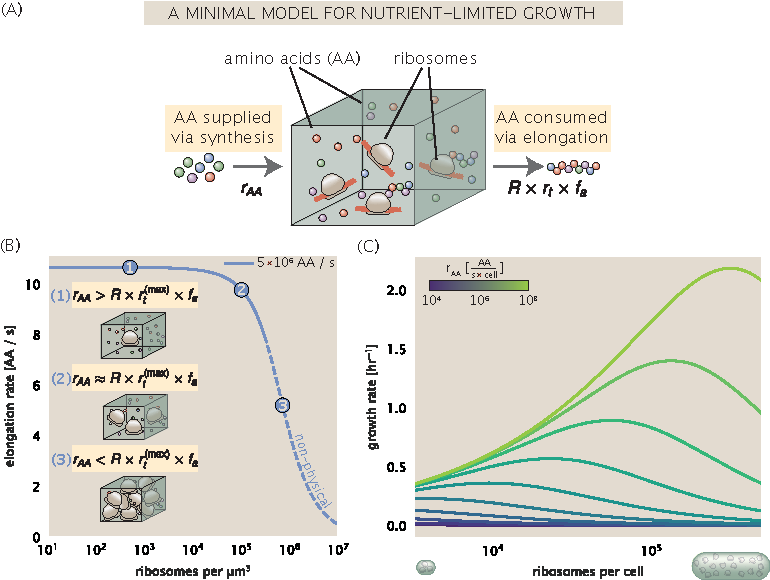
\includegraphics{main_figs/elongation_model.pdf}
        \caption{\textbf{A minimal model of growth rate control under
        nutrient limitation.} (A) We consider a unit volume of cellular material
        composed of amino acids (colored spheres) provided at a supply rate
        $r_{AA}$. These amino acids are polymerized by a pool of ribosomes
        (brown blobs) at a rate $r_t \times R \times f_a$, where $r_t$ is the
        elongation rate, $R$ is the ribosome copy number in the unit volume, and
        $f_a$ is the fraction of those ribosomes actively translating. (B) The
        observed elongation rate is plotted as a function of ribosomes in a unit
        volume \textmu m$^3$. The three points correspond to three regimes of
        ribosome copy numbers and are shown schematically on the left-hand side.
        The region of the curve shown as dashed lines represents a non-physical
        copy number, but is shown for illustrative purposes. This curve was
        generated using the parameters $r_{AA} = 5 \times 10^6$ AA / s, $K_D =
        5$ mM, and $r_t^\text{(max)} = 17.1$ AA / s. (C) The cellular growth
        rate is plotted as a function of total cellular ribosome copy number for
        different cellular amino acid supply rates, with blue and green curves
        corresponding to low and high supply rates, repsectively. As the
        ribosome copy number is increased, so too is the cell volume and total
        protein abundance. We direct the reader to the Suppemental Information
        for discussion  on the inference of the realtionship between cell
        volume, number of peptide bonds, and ribosome copy number.}
        \label{fig:elongation_rate_model}
    }
\end{figure}

\subsection{Optimal Growth Rate, Ribosomal Content, and Cell Size Depend on Nutrient
Availability and Metabolic Capacity.}

To relate elongation rate to growth rate, we constrain the set of parameters
based on our available proteomic measurements; namely, we restrict the values of
$R$, $N_{pep}$, and cell size to those associated with the amalgamated proteomic
data (described in Appendix \nameref{sec:estimate_protein_per_cell}). We then
consider how changes in the nutrient conditions, through the parameter $r_{AA}$,
influence the maximum growth rate as determined by \EQ{lambda_limit}.
\FIG{elongation_rate_model}(C) shows how the observed growth rate depends on the
rate of amino acid supply $r_{AA}$ as a function of the cellular ribosome copy
number. A feature immediately apparent is the presence of a maximal growth rate
whose dependence on $R$ (and consequently, the cell size) increases with
increasing $r_{AA}$. Importantly, however, there is an optimum set of $R$,
$N_{pep}$, and $V$ that are strictly dependent on the value of $r_{AA}$.
Increasing the ribosomal concentration beyond the cell's metabolic capacity has
the adverse consequence of depleting the supply of amino acids and a concomitant
decrease in the elongation rate $r_t$ [\FIG{elongation_rate_model}(B)].

Also of note is the growth rate profiles shown for low amino acid supply rates
[purple and blue lines in \FIG{elongation_rate_model}(C)], representing growth
in nutrient-poor media. In these conditions, there no longer exists a peak in
growth, at least in the range of physiologically-relevant  ribosome copy
numbers. Instead, cells limit their pool of actively translating ribosomes  by
decreasing $f_a$ \citep{dai2016}, which would help maintain the pool of
available amino acids $[AA]_\text{eff}$ and increase the achievable elongation
rate. This observation is in agreement with the central premise of the cellular
resource allocation principle proposed by \cite{scott2010,
klumpp2009,klumpp2014} and \cite{hui2015}.
